%!TEX root = book.tex
\chapter{Linear Regression}

\index{Linear Regression}
 
Trong bài này, tôi sẽ giới thiệu một trong những thuật toán cơ bản nhất (và đơn giản nhất) của Machine Learning. Đây là một thuật toán \textit{Supervised learning} có tên {\textbf{Linear Regression}} (Hồi Quy Tuyến Tính). Bài toán này đôi khi được gọi là \textit{Linear Fitting} (trong thống kê) hoặc \textit{Linear Least Square}. 

\section{Giới thiệu}
 
Quay lại \href{http://machinelearningcoban.com/2016/12/27/categories/#regression-hoi-quy}{ví dụ đơn giản được nêu trong bài trước}: một căn nhà rộng $x_1 ~ \text{m}^2$, có $x_2$ phòng ngủ và cách trung tâm thành phố $x_3~ \text{km}$ có giá là bao nhiêu. Giả sử chúng ta đã có số liệu thống kê từ 1000 căn nhà trong thành phố đó, liệu rằng khi có một căn nhà mới với các thông số về diện tích, số phòng ngủ và khoảng cách tới trung tâm, chúng ta có thể dự đoán được giá của căn nhà đó không? Nếu có thì hàm dự đoán $y = f(\mathbf{x}) $ sẽ có dạng như thế nào. Ở đây $\mathbf{x} = [x_1, x_2, x_3] $ là một vector hàng chứa thông tin \textit{input}, $y$ là một số vô hướng (scalar) biểu diễn \textit{output} (tức giá của căn nhà trong ví dụ này). 
 
\textbf{Lưu ý về ký hiệu toán học:} \textit{trong các bài viết của tôi, các số vô hướng được biểu diễn bởi các chữ cái viết ở dạng không in đậm, có thể viết hoa, ví dụ $x_1, N, y, k$. Các vector được biểu diễn bằng các chữ cái thường in đậm, ví dụ $\mathbf{y}, \mathbf{x}_1 $. Các ma trận được biểu diễn bởi các chữ viết hoa in đậm, ví dụ $\mathbf{X, Y, W} $.} 
 
Một cách đơn giản nhất, chúng ta có thể thấy rằng: i) diện tích nhà càng lớn thì giá nhà càng cao; ii) số lượng phòng ngủ càng lớn thì giá nhà càng cao; iii) càng xa trung tâm thì giá nhà càng giảm. Một hàm số đơn giản nhất có thể mô tả mối quan hệ giữa giá nhà và 3 đại lượng đầu vào là:  
\begin{equation}
\label{eqn:linearregression}
y \approx   \hat{y} = f(\mathbf{x}) =w_1 x_1 + w_2 x_2 + w_3 x_3 + w_0 
\end{equation}
trong đó, $w_1, w_2, w_3, w_0$ là các hằng số,  $w_0$ còn được gọi là bias. Mối quan hệ $y \approx f(\mathbf{x})$ bên trên là một mối quan hệ tuyến tính (linear). Bài toán chúng ta đang làm là một bài toán thuộc loại regression. Bài toán đi tìm các hệ số tối ưu $ \\{w_1, w_2, w_3, w_0 \\}$ chính vì vậy được gọi là bài toán Linear Regression.  
 
\textbf{Chú ý 1:} $y$ là giá trị thực của \textit{outcome} (dựa trên số liệu thống kê chúng ta có trong tập \textit{training data}), trong khi $\hat{y}$ là giá trị mà mô hình Linear Regression dự đoán được. Nhìn chung, $y$ và $\hat{y}$ là hai giá trị khác nhau do có sai số mô hình, tuy nhiên, chúng ta mong muốn rằng sự khác nhau này rất nhỏ. 
 
\textbf{Chú ý 2:} \textit{Linear} hay \textit{tuyến tính} hiểu một cách đơn giản là \textit{thẳng, phẳng}. Trong không gian hai chiều, một hàm số được gọi là \textit{tuyến tính} nếu đồ thị của nó có dạng một \textit{đường thẳng}. Trong không gian ba chiều, một hàm số được goi là \textit{tuyến tính} nếu đồ thị của nó có dạng một \textit{mặt phẳng}. Trong không gian nhiều hơn 3 chiều, khái niệm \textit{mặt phẳng} không còn phù hợp nữa, thay vào đó, một khái niệm khác ra đời được gọi là \textit{siêu mặt phẳng} (\textit{hyperplane}). Các hàm số tuyến tính là các hàm đơn giản nhất, vì chúng thuận tiện trong việc hình dung và tính toán. Chúng ta sẽ được thấy trong các bài viết sau, \textit{tuyến tính} rất quan trọng và hữu ích trong các bài toán Machine Learning. Kinh nghiệm cá nhân tôi cho thấy, trước khi hiểu được các thuật toán \textit{phi tuyến} (non-linear, không phẳng), chúng ta cần nắm vững các kỹ thuật cho các mô hình \textit{tuyến tính}. 
 
 
 
 
 
\section{Phân tích toán học}
 
 
 
 
\subsection{Dạng của Linear Regression }
 
Trong phương trình $(1)$ phía trên, nếu chúng ta đặt $\mathbf{w} = [w_0, w_1, w_2, w_3]^T = $ là vector (cột) hệ số cần phải tối ưu và $\mathbf{\bar{x}} = [1, x_1, x_2, x_3]$ (đọc là \textit{x bar} trong tiếng Anh) là vector (hàng) dữ liệu đầu vào \textit{mở rộng}. Số $1$ ở đầu được thêm vào để phép tính đơn giản hơn và thuận tiện cho việc tính toán. Khi đó, phương trình (1) có thể được viết lại dưới dạng: 
$$y \approx \mathbf{\bar{x}}\mathbf{w} = \hat{y}$$ 
 
Chú ý rằng $\mathbf{\bar{x}}$ là một vector hàng. (\href{http://machinelearningcoban.com/math/#luu-y-ve-ky-hieu}{Xem thêm về ký hiệu vector hàng và cột tại đây}) 
 
 
 
\subsection{Sai số dự đoán }
 
Chúng ta mong muốn rằng sự sai khác $e$ giữa giá trị thực $y$ và giá trị dự đoán $\hat{y}$ (đọc là \textit{y hat} trong tiếng Anh) là nhỏ nhất. Nói cách khác, chúng ta muốn giá trị sau đây càng nhỏ càng tốt:  
 \begin{equation*}
\frac{1}{2}e^2 = \frac{1}{2}(y - \hat{y})^2 = \frac{1}{2}(y - \mathbf{\bar{x}}\mathbf{w})^2 
\end{equation*}
 trong đó hệ số $\frac{1}{2} $ (\textit{lại}) là để thuận tiện cho việc tính toán (khi tính đạo hàm thì số $\frac{1}{2} $ sẽ bị triệt tiêu). Chúng ta cần $e^2$ vì $e = y - \hat{y} $ có thể là một số âm, việc nói $e$ nhỏ nhất sẽ không đúng vì khi $e = - \infty$ là rất nhỏ nhưng sự sai lệch là rất lớn. Bạn đọc có thể tự đặt câu hỏi: \textbf{tại sao không dùng trị tuyệt đối $ \|e\| $ mà lại dùng bình phương $e^2$ ở đây?} Câu trả lời sẽ có ở phần sau.  
 
 
 
 
 
 
\subsection{Hàm mất mát}
 
Điều tương tự xảy ra với tất cả các cặp \textit{(input, outcome)} $ (\mathbf{x}_i, y_i), i = 1, 2, \dots, N $, với $N$ là số lượng dữ liệu quan sát được. Điều chúng ta muốn, tổng sai số là nhỏ nhất, tương đương với việc tìm $ \mathbf{w} $ để hàm số sau đạt giá trị nhỏ nhất: 
\begin{equation}
\label{eqn:linearregression_loss} 
 \mathcal{L}(\mathbf{w}) = \frac{1}{2}\sum_{i=1}^N (y_i - \mathbf{\bar{x}_i}\mathbf{w})^2
\end{equation}  
 
Hàm số $\mathcal{L}(\mathbf{w}) $ được gọi là \textbf{hàm mất mát} (loss function) của bài toán Linear Regression. Chúng ta luôn mong muốn rằng sự mất mát (sai số) là nhỏ nhất, điều đó đồng nghĩa với việc  tìm vector hệ số $ \mathbf{w} $  sao cho  
giá trị của hàm mất mát này càng nhỏ càng tốt. Giá trị của $\mathbf{w}$ làm cho hàm mất mát đạt giá trị nhỏ nhất được gọi là \textit{điểm tối ưu} (optimal point), ký hiệu: 
 
$$ \mathbf{w}^* = \arg\min_{\mathbf{w}} \mathcal{L}(\mathbf{w})  $$  
 
Trước khi đi tìm lời giải, chúng ta đơn giản hóa phép toán trong phương trình hàm mất mát \eqref{eqn:linearregression_loss}. Đặt $\mathbf{y} = [y_1; y_2; \dots; y_N]$ là một vector cột chứa tất cả các \textit{output} của \textit{training data}; $ \mathbf{\bar{X}} = [\mathbf{\bar{x}}_1; \mathbf{\bar{x}}_2; \dots; \mathbf{\bar{x}}_N ] $ là ma trận dữ liệu đầu vào (mở rộng) mà mỗi hàng của nó là một điểm dữ liệu. Khi đó hàm số mất mát $\mathcal{L}(\mathbf{w})$ được viết dưới dạng ma trận đơn giản hơn: 
\begin{equation}
\label{eqn:linearregression_loss_mat}
\mathcal{L}(\mathbf{w})  
= \frac{1}{2}\sum_{i=1}^N (y_i - \mathbf{\bar{x}}_i\mathbf{w})^2 
= \frac{1}{2} \|\mathbf{y} - \mathbf{\bar{X}}\mathbf{w} \|_2^2  
\end{equation} 
với $ \| \mathbf{z} \|_2 $ là Euclidean norm (chuẩn Euclid, hay khoảng cách Euclid), nói cách khác $ \| \mathbf{z} \|_2^2 $ là tổng của bình phương mỗi phần tử của vector $\mathbf{z}$. Tới đây, ta đã có một dạng đơn giản của hàm mất mát được viết như phương trình \eqref{eqn:linearregression_loss_mat}. 
 
 
 
 
\subsection{Nghiệm cho bài toán Linear Regression}
 
\textbf{Cách phổ biến nhất để tìm nghiệm cho một bài toán tối ưu (chúng ta đã biết từ khi học cấp 3) là giải phương trình đạo hàm (gradient) bằng 0!} Tất nhiên đó là khi việc tính đạo hàm và việc giải phương trình đạo hàm bằng 0 không quá phức tạp. Thật may mắn, với các mô hình tuyến tính, hai việc này là khả thi.  
 
Đạo hàm theo $\mathbf{w} $ của hàm mất mát là:  
$$ 
\frac{\partial{\mathcal{L}(\mathbf{w})}}{\partial{\mathbf{w}}}  
= \mathbf{\bar{X}}^T(\mathbf{\bar{X}}\mathbf{w} - \mathbf{y})  
$$ 
 
Các bạn có thể tham khảo bảng đạo hàm theo vector hoặc ma trận của một hàm số trong \href{https://ccrma.stanford.edu/~dattorro/matrixcalc.pdf}{mục D.2 của tài liệu này}. \textit{Đến đây tôi xin quay lại câu hỏi ở phần Sai số dự đoán phía trên về việc tại sao không dùng trị tuyệt đối mà lại dùng bình phương. Câu trả lời là hàm bình phương có đạo hàm tại mọi nơi, trong khi hàm trị tuyệt đối thì không (đạo hàm không xác định tại 0)}. 
 
Phương trình đạo hàm bằng 0 tương đương với:  
\begin{equation}
\label{eqn:linearregression_gradient}
\mathbf{\bar{X}}^T\mathbf{\bar{X}}\mathbf{w} = \mathbf{\bar{X}}^T\mathbf{y} \triangleq \mathbf{b}  
\end{equation}
(ký hiệu $\mathbf{\bar{X}}^T\mathbf{y} \triangleq \mathbf{b} $ nghĩa là \textit{đặt} $\mathbf{\bar{X}}^T\mathbf{y}$ \textit{bằng} $\mathbf{b}$ ). 
 
Nếu ma trận vuông $ \mathbf{A} \triangleq \mathbf{\bar{X}}^T\mathbf{\bar{X}}$ khả nghịch (non-singular hay inversable) thì phương trình $(4)$ có nghiệm duy nhất: $ \mathbf{w} = \mathbf{A}^{-1}\mathbf{b}  $. 
 
Vậy nếu ma trận $\mathbf{A} $ không khả nghịch (có định thức bằng 0) thì sao? Nếu các bạn vẫn nhớ các kiến thức về hệ phương trình tuyến tính, trong trường hợp này thì hoặc phương trinh \eqref{eqn:linearregression_gradient} vô nghiệm, hoặc làp  
nó 
có vô số nghiệm. Khi đó, chúng ta sử dụng khái niệm \href{https://vi.wikipedia.org/wiki/Giả_nghịch_đảo_Moore–Penrose}{\textit{giả nghịch đảo}} $ \mathbf{A}^{\dagger} $ (đọc là \textit{A dagger} trong tiếng Anh). (\textit{Giả nghịch đảo (pseudo inverse) là trường hợp tổng quát của nghịch đảo khi ma trận không khả nghịch hoặc thậm chí không vuông. Trong khuôn khổ bài viết này, tôi xin phép được lược bỏ phần này, nếu các bạn thực sự quan tâm, tôi sẽ viết một bài khác chỉ nói về giả nghịch đảo. Xem thêm: \href{http://www.sci.utah.edu/~gerig/CS6640-F2012/Materials/pseudoinverse-cis61009sl10.pdf}{Least Squares, Pseudo-Inverses, PCA \& SVD}.}) 
 
Với khái niệm giả nghịch đảo, điểm tối ưu của bài toán Linear Regression có dạng: 
\begin{equation}
\label{eqn:linearregression_solution}
\mathbf{w} = \mathbf{A}^{\dagger}\mathbf{b} = (\mathbf{\bar{X}}^T\mathbf{\bar{X}})^{\dagger} \mathbf{\bar{X}}^T\mathbf{y} 
\end{equation} 
 
 
 
\section{Ví dụ trên Python}
 
 
\subsection{Bài toán}
 
Trong phần này, tôi sẽ chọn một ví dụ đơn giản về việc giải bài toán Linear Regression trong Python. Tôi cũng sẽ so sánh nghiệm của bài toán khi giải theo phương trình \eqref{eqn:linearregression_solution} và nghiệm tìm được khi dùng thư viện \href{http://scikit-learn.org/stable/}{scikit-learn} của Python. (\textit{Đây là thư viện Machine Learning được sử dụng rộng rãi trong Python}). Trong ví dụ này, dữ liệu đầu vào chỉ có 1 giá trị (1 chiều) để thuận tiện cho việc minh hoạ trong mặt phẳng.  
 
Chúng ta có 1 bảng dữ liệu về chiều cao và cân nặng của 15 người như trong Bảng \ref{tab:height_weight}. 
 
 
\begin{table}[h!]
\centering
\caption{Bảng dữ liệu về chiều cao và cân nặng của 15 người}
\label{tab:height_weight}
\begin{tabular}{|c|c|c|c|}
\hline
\textbf{Chiều cao (cm)} & \textbf{Cân nặng (kg)} & \textbf{Chiều cao (cm)} & \textbf{Cân nặng (kg)} \\ \hline
147                     & 49                     & 168                     & 60                     \\ \hline
150                     & 50                     & 170                     & 72                     \\ \hline
153                     & 51                     & 173                     & 63                     \\ \hline
155                     & 52                     & 175                     & 64                     \\ \hline
158                     & 54                     & 178                     & 66                     \\ \hline
160                     & 56                     & 180                     & 67                     \\ \hline
163                     & 58                     & 183                     & 68                     \\ \hline
165                     & 59                     &                         &                        \\ \hline
\end{tabular}
\end{table}

Bài toán đặt ra là: liệu có thể dự đoán cân nặng của một người dựa vào chiều cao của họ không? (\textit{Trên thực tế, tất nhiên là không, vì cân nặng còn phụ thuộc vào nhiều yếu tố khác nữa, thể tích chẳng hạn}). Vì blog này nói về các thuật toán Machine Learning đơn giản nên tôi sẽ giả sử rằng chúng ta có thể dự đoán được. 
 
Chúng ta có thể thấy là cân nặng sẽ tỉ lệ thuận với chiều cao (càng cao càng nặng), nên có thể sử dụng Linear Regression model cho việc dự đoán này. Để kiểm tra độ chính xác của model tìm được, chúng ta sẽ giữ lại cột 155 và 160 cm để kiểm thử, các cột còn lại được sử dụng để huấn luyện (train) model. 
 
 
\subsection{Hiển thị dữ liệu trên đồ thị}
Trước tiên, chúng ta cần có hai thư viện \href{http://www.numpy.org/}{numpy} cho đại số tuyến tính và \href{http://matplotlib.org/}{matplotlib} cho việc vẽ hình.  
 
 
\begin{lstlisting}[language=Python]
# To support both python 2 and python 3 
from __future__ import division, print_function, unicode_literals 
import numpy as np  
import matplotlib.pyplot as plt 
\end{lstlisting}
 
Tiếp theo, chúng ta khai báo và biểu diễn dữ liệu trên một đồ thị. 
 
 
\begin{lstlisting}[language=Python]
# height (cm) 
X = np.array([[147, 150, 153, 158, 163, 165, 168, 170, 173, 175, 178, 180, 183]]).T 
# weight (kg) 
y = np.array([[ 49, 50, 51,  54, 58, 59, 60, 62, 63, 64, 66, 67, 68]]).T 
# Visualize data  
plt.plot(X, y, 'ro') 
plt.axis([140, 190, 45, 75]) 
plt.xlabel('Height (cm)') 
plt.ylabel('Weight (kg)') 
plt.show() 
\end{lstlisting}
 
 
% <div class="imgcap"> 
% <img src ="/assets/LR/output_3_0.png" align = "center"> 
% </div> 
 
 \begin{figure}
 	\centering	
 	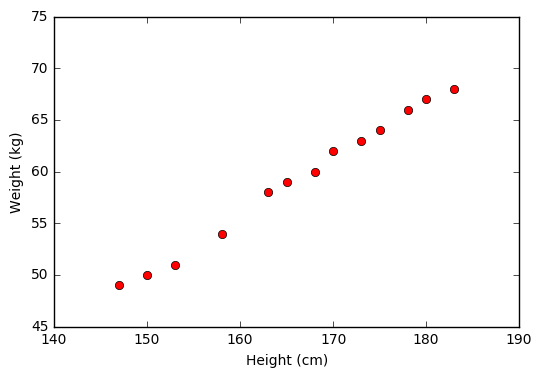
\includegraphics[width = .6\textwidth]{../LR/output_3_0.png}
 	\caption{ Phân bố của dữ liệu trong ví dụ có dạng đường thẳng}
 	\label{fig:linearregression_distribution}
 \end{figure}
 
Từ đồ thị trong Hình \ref{fig:linearregression_distribution} ta thấy rằng dữ liệu được sắp xếp gần như theo 1 đường thẳng, vậy mô hình Linear Regression nhiều khả năng sẽ cho kết quả tốt: 
 
(cân nặng) = \pythoninline{w\_1}*(chiều cao) + \pythoninline{w\_0} 
 
 
\subsection{Nghiệm theo công thức}
 
Tiếp theo, chúng ta sẽ tính toán các hệ số \pythoninline{w_1} và \pythoninline{w_0} dựa vào công thức $(5)$. Chú ý: giả nghịch đảo của một ma trận \pythoninline{A} trong Python sẽ được tính bằng \pythoninline{numpy.linalg.pinv(A)}, \pythoninline{pinv} là từ viết tắt của \textit{pseudo inverse}. 
 
\begin{lstlisting}[language=Python]
# Building Xbar  
one = np.ones((X.shape[0], 1)) 
Xbar = np.concatenate((one, X), axis = 1) 
 
# Calculating weights of the fitting line  
A = np.dot(Xbar.T, Xbar) 
b = np.dot(Xbar.T, y) 
w = np.dot(np.linalg.pinv(A), b) 
print('w = ', w) 
# Preparing the fitting line  
w_0 = w[0][0] 
w_1 = w[1][0] 
x0 = np.linspace(145, 185, 2) 
y0 = w_0 + w_1*x0 
 
# Drawing the fitting line  
plt.plot(X.T, y.T, 'ro')     # data  
plt.plot(x0, y0)               # the fitting line 
plt.axis([140, 190, 45, 75]) 
plt.xlabel('Height (cm)') 
plt.ylabel('Weight (kg)') 
plt.show() 
 
\end{lstlisting}
 
\begin{lstlisting}[language=Python]
w =  [[-33.73541021] 
 [  0.55920496]] 
\end{lstlisting}
 
 


\begin{figure}
	\centering
	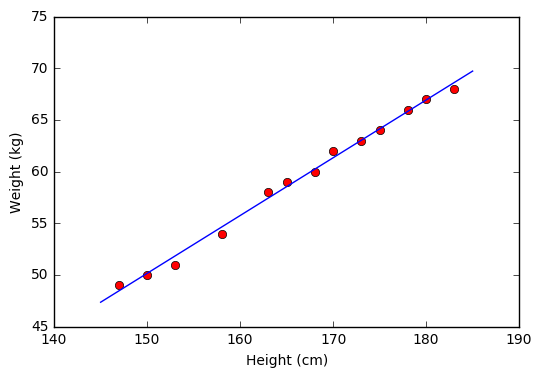
\includegraphics[width = .6\textwidth]{../LR/output_5_1.png}
	\caption{Minh họa nghiệm của ví dụ}
\end{figure}
 
Từ đồ thị bên trên ta thấy rằng các điểm dữ liệu màu đỏ nằm khá gần đường thẳng dự đoán màu xanh. Vậy mô hình Linear Regression hoạt động tốt với tập dữ liệu \textit{training}. Bây giờ, chúng ta sử dụng mô hình này để dự đoán cân nặng của hai người có chiều cao 155 và 160 cm mà chúng ta đã không dùng khi tính toán nghiệm. 
 
 
\begin{lstlisting}[language=Python]
y1 = w_1*155 + w_0 
y2 = w_1*160 + w_0 
 
print( 'Predict weight of person 155 cm: %.2f (kg), real number: 52 (kg)'  %(y1) ) 
print( 'Predict weight of person 160 cm: %.2f (kg), real number: 56 (kg)'  %(y2) ) 
\end{lstlisting}
 

\begin{lstlisting}[language=Python]
Predict weight of person 155 cm: 52.94 (kg), real number: 52 (kg) 
Predict weight of person 160 cm: 55.74 (kg), real number: 56 (kg) 
\end{lstlisting}
 
 
Chúng ta thấy rằng kết quả dự đoán khá gần với số liệu thực tế. 
 
 
\subsection{Nghiệm theo thư viện scikit-learn}
 
Tiếp theo, chúng ta sẽ sử dụng thư viện scikit-learn của Python để tìm nghiệm.  
 
 
\begin{lstlisting}[language=Python]
from sklearn import datasets, linear_model 
 
# fit the model by Linear Regression 
regr = linear_model.LinearRegression(fit_intercept=False) # fit_intercept = False for calculating the bias 
regr.fit(Xbar, y) 
 
# Compare two results 
print( 'Solution found by scikit-learn  : ', regr.coef_ ) 
print( 'Solution found by (5): ', w.T) 
\end{lstlisting}
 
\begin{lstlisting}[language=Python]
    Solution found by scikit-learn  :  [[  -33.73541021 0.55920496]] 
    Solution found by (5):  [[  -33.73541021 0.55920496 ]] 
\end{lstlisting}
 
Chúng ta thấy rằng hai kết quả thu được như nhau! (\textit{Nghĩa là tôi đã không mắc lỗi nào trong cách tìm nghiệm ở phần trên}) 
 
\href{https://github.com/tiepvupsu/tiepvupsu.github.io/blob/master/assets/LR/LR.ipynb}{Source code Jupyter Notebook cho bài này.} 
 
 
 
\section{Thảo luận}
 
 
\subsection{Các bài toán có thể giải bằng Linear Regression}
Hàm số $y \approx f(\mathbf{x})= \mathbf{w}^T\mathbf{x}$ là một hàm tuyến tính theo cả $ \mathbf{w}$ và $\mathbf{x}$. Trên thực tế, Linear Regression có thể áp dụng cho các mô hình chỉ cần tuyến tính theo $\mathbf{w}$. Ví dụ: 
$$ 
y \approx w_1 x_1 + w_2 x_2 + w_3 x_1^2 +  w_4 \sin(x_2) + w_5 x_1x_2 + w_0 
$$ 
là một hàm tuyến tính theo $\mathbf{w}$ và vì vậy cũng có thể được giải bằng Linear Regression. Với mỗi dữ liệu đầu vào $\mathbf{x}=[x_1; x_2] $, chúng ta tính toán dữ liệu mới $\tilde{\mathbf{x}} = [x_1, x_2, x_1^2, \sin(x_2), x_1x_2]$ (đọc là \textit{x tilde} trong tiếng Anh) rồi áp dụng Linear Regression với dữ liệu mới này.  
 
Xem thêm ví dụ về \href{http://www.varsitytutors.com/hotmath/hotmath_help/topics/quadratic-regression}{Quadratic Regression} (Hồi Quy Bậc Hai). 
% <div class="imgcap"> 
% <div > 
%     <img src ="http://www.varsitytutors.com/assets/vt-hotmath-legacy/hotmath_help/topics/quadratic-regression/f-qr-1-1.gif"  width = "300"></a> 
% </div> 
% <div class="thecap"> Quadratic Regression (Nguồn: <a href = "http://www.varsitytutors.com/hotmath/hotmath_help/topics/quadratic-regression"> Quadratic Regression</a>) <br></div> 
% </div> 
 
 \begin{figure}
   \centering
   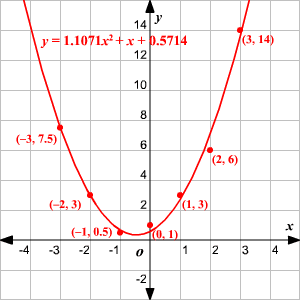
\includegraphics[width = .4\textwidth]{../LR/qr.png}
   \caption{Quadratic Regression (Nguồn: \href{http://www.varsitytutors.com/hotmath/hotmath_help/topics/quadratic-regression}{Quadratic Regression})}
   \label{fig:linearregression_qr}
 \end{figure}
 
\subsection{Hạn chế của Linear Regression}
 
Hạn chế đầu tiên của Linear Regression là nó rất \textbf{nhạy cảm với nhiễu} (sensitive to noise). Trong ví dụ về mối quan hệ giữa chiều cao và cân nặng bên trên, nếu có chỉ 
một cặp dữ liệu \textit{nhiễu} (150 cm, 90kg) thì kết quả sẽ sai khác đi rất nhiều (Xem Hình \ref{fig:linearregression_noise}). 
% <div class="imgcap"> 
% <img src ="/assets/LR/output_13_1.png" align = "center"> 
% </div> 
 
 \begin{figure}
 	\centering
 	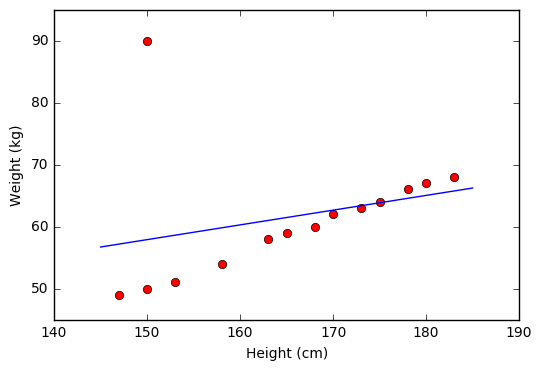
\includegraphics[width = .6\textwidth]{../LR/output_13_1.png}
 	\caption{Linear Regression rất nhạy cảm với nhiễu}
 	\label{fig:linearregression_noise}
 \end{figure}
Vì vậy, trước khi thực hiện Linear Regression, các nhiễu (\textit{outlier}) cần 
 phải được loại bỏ. Bước này được gọi là tiền xử lý (pre-processing). 
 
Hạn chế thứ hai của Linear Regression là nó \textbf{không biễu diễn được các mô hình phức tạp}. Mặc dù trong phần trên, chúng ta thấy rằng phương pháp này có thể được áp dụng nếu quan hệ giữa \textit{outcome} và \textit{input} không nhất thiết phải là tuyến tính, nhưng mối quan hệ này vẫn đơn giản nhiều so với các mô hình thực tế. Hơn nữa, chúng ta sẽ tự hỏi: làm thế nào để xác định được các hàm $x_1^2, \sin(x_2), x_1x_2$ như ở trên?! 
 
 
\subsection{Các phương pháp tối ưu}
Linear Regression là một mô hình đơn giản, lời giải cho phương trình đạo hàm bằng 0 cũng khá đơn giản. \textit{Trong hầu hết các trường hợp, chúng ta không thể giải được phương trình đạo hàm bằng 0.} 
 
Nhưng có một điều chúng ta nên nhớ, \textbf{còn tính được đạo hàm là còn có cơ hội}. 
 
 
 
 
\section{Tài liệu tham khảo}
 \begin{enumerate}
 	\item  \href{https://en.wikipedia.org/wiki/Linear_regression}{Linear Regression - Wikipedia}

 	\item  \href{http://machinelearningmastery.com/simple-linear-regression-tutorial-for-machine-learning/}{Simple Linear Regression Tutorial for Machine Learning} 

 	\item  \href{http://www.sci.utah.edu/~gerig/CS6640-F2012/Materials/pseudoinverse-cis61009sl10.pdf}{Least Squares, Pseudo-Inverses, PCA \& SVD} 
 \end{enumerate}
